\documentclass[11pt]{article}
% Shared preamble for the NSE working-paper series (Mrigank Sahi).
% Usage in each paper: % Shared preamble for the NSE working-paper series (Mrigank Sahi).
% Usage in each paper: % Shared preamble for the NSE working-paper series (Mrigank Sahi).
% Usage in each paper: \input{../common/preamble.tex}
\usepackage[T1]{fontenc}
\usepackage[utf8]{inputenc}
\usepackage{lmodern}
\usepackage{microtype}
\usepackage[a4paper,margin=1in]{geometry}
\usepackage{amsmath,amssymb}
\usepackage{booktabs}
\usepackage{tabularx}
\usepackage{siunitx}
\sisetup{group-separator={,},round-mode=places,round-precision=3}
\usepackage{graphicx}
\usepackage{xcolor}
\usepackage{caption}
\captionsetup{font=small,labelfont=bf}
\usepackage{enumitem}
\setlist{nosep,leftmargin=*}
\usepackage[framemethod=TikZ]{mdframed}
\usepackage[numbers,sort&compress]{natbib}
\usepackage[colorlinks=true,linkcolor=black,citecolor=blue!50!black,urlcolor=blue!50!black]{hyperref}

\newcommand{\ghbase}{https://github.com/mriganksahi-beep}
\newcommand{\authorline}{Mrigank Sahi\\\small Independent Researcher, New Delhi\\\small\texttt{mriganksahi@gmail.com}}

% Standard disclosure box. Every paper fills all five fields.
% #1 sample/period status, #2 position in test tally, #3 costs,
% #4 point-in-time limits, #5 anything else the reader must know
\newcommand{\caveatsbox}[5]{%
\begin{mdframed}[backgroundcolor=gray!8,linecolor=gray!50,innertopmargin=6pt,innerbottommargin=6pt]
\small\textbf{Read before interpreting results.}
\begin{itemize}
\item \textbf{Sample.} #1
\item \textbf{Multiple testing.} #2
\item \textbf{Costs.} #3
\item \textbf{Point-in-time universe.} #4
\item \textbf{Other.} #5
\end{itemize}
\end{mdframed}}

% Standard AI-assistance statement (identical across the series).
\newcommand{\aistatement}{%
\paragraph{Use of AI tools.} Code for this project was written with the assistance of
an AI coding assistant (Anthropic's Claude), working to specifications set by the
author, and the manuscript was drafted with the same assistance. The author designed
the research questions and decision rules and ran the main analyses. Some diagnostics
added during revision were computed by the assistant from archived run outputs; these
are labelled as revision diagnostics in the text. The author reviewed all code and
text and takes full responsibility for the content.}

% Standard data/code availability statement.
\newcommand{\availability}[1]{%
\paragraph{Data and code availability.} Code: \url{#1}. The point-in-time panel
construction is documented in \url{\ghbase/indian-equity-research/tree/main/data_pipeline}.
Price data from Yahoo Finance and index-membership snapshots from a licensed vendor
are not redistributed; the repository contains the scripts to rebuild the panel.}

% Placeholder for anything awaiting the author's confirmation. Renders red so it
% cannot survive into a posted PDF unnoticed.
\newcommand{\verify}[1]{\textcolor{red}{\textbf{[VERIFY: #1]}}}

\usepackage[T1]{fontenc}
\usepackage[utf8]{inputenc}
\usepackage{lmodern}
\usepackage{microtype}
\usepackage[a4paper,margin=1in]{geometry}
\usepackage{amsmath,amssymb}
\usepackage{booktabs}
\usepackage{tabularx}
\usepackage{siunitx}
\sisetup{group-separator={,},round-mode=places,round-precision=3}
\usepackage{graphicx}
\usepackage{xcolor}
\usepackage{caption}
\captionsetup{font=small,labelfont=bf}
\usepackage{enumitem}
\setlist{nosep,leftmargin=*}
\usepackage[framemethod=TikZ]{mdframed}
\usepackage[numbers,sort&compress]{natbib}
\usepackage[colorlinks=true,linkcolor=black,citecolor=blue!50!black,urlcolor=blue!50!black]{hyperref}

\newcommand{\ghbase}{https://github.com/mriganksahi-beep}
\newcommand{\authorline}{Mrigank Sahi\\\small Independent Researcher, New Delhi\\\small\texttt{mriganksahi@gmail.com}}

% Standard disclosure box. Every paper fills all five fields.
% #1 sample/period status, #2 position in test tally, #3 costs,
% #4 point-in-time limits, #5 anything else the reader must know
\newcommand{\caveatsbox}[5]{%
\begin{mdframed}[backgroundcolor=gray!8,linecolor=gray!50,innertopmargin=6pt,innerbottommargin=6pt]
\small\textbf{Read before interpreting results.}
\begin{itemize}
\item \textbf{Sample.} #1
\item \textbf{Multiple testing.} #2
\item \textbf{Costs.} #3
\item \textbf{Point-in-time universe.} #4
\item \textbf{Other.} #5
\end{itemize}
\end{mdframed}}

% Standard AI-assistance statement (identical across the series).
\newcommand{\aistatement}{%
\paragraph{Use of AI tools.} Code for this project was written with the assistance of
an AI coding assistant (Anthropic's Claude), working to specifications set by the
author, and the manuscript was drafted with the same assistance. The author designed
the research questions and decision rules and ran the main analyses. Some diagnostics
added during revision were computed by the assistant from archived run outputs; these
are labelled as revision diagnostics in the text. The author reviewed all code and
text and takes full responsibility for the content.}

% Standard data/code availability statement.
\newcommand{\availability}[1]{%
\paragraph{Data and code availability.} Code: \url{#1}. The point-in-time panel
construction is documented in \url{\ghbase/indian-equity-research/tree/main/data_pipeline}.
Price data from Yahoo Finance and index-membership snapshots from a licensed vendor
are not redistributed; the repository contains the scripts to rebuild the panel.}

% Placeholder for anything awaiting the author's confirmation. Renders red so it
% cannot survive into a posted PDF unnoticed.
\newcommand{\verify}[1]{\textcolor{red}{\textbf{[VERIFY: #1]}}}

\usepackage[T1]{fontenc}
\usepackage[utf8]{inputenc}
\usepackage{lmodern}
\usepackage{microtype}
\usepackage[a4paper,margin=1in]{geometry}
\usepackage{amsmath,amssymb}
\usepackage{booktabs}
\usepackage{tabularx}
\usepackage{siunitx}
\sisetup{group-separator={,},round-mode=places,round-precision=3}
\usepackage{graphicx}
\usepackage{xcolor}
\usepackage{caption}
\captionsetup{font=small,labelfont=bf}
\usepackage{enumitem}
\setlist{nosep,leftmargin=*}
\usepackage[framemethod=TikZ]{mdframed}
\usepackage[numbers,sort&compress]{natbib}
\usepackage[colorlinks=true,linkcolor=black,citecolor=blue!50!black,urlcolor=blue!50!black]{hyperref}

\newcommand{\ghbase}{https://github.com/mriganksahi-beep}
\newcommand{\authorline}{Mrigank Sahi\\\small Independent Researcher, New Delhi\\\small\texttt{mriganksahi@gmail.com}}

% Standard disclosure box. Every paper fills all five fields.
% #1 sample/period status, #2 position in test tally, #3 costs,
% #4 point-in-time limits, #5 anything else the reader must know
\newcommand{\caveatsbox}[5]{%
\begin{mdframed}[backgroundcolor=gray!8,linecolor=gray!50,innertopmargin=6pt,innerbottommargin=6pt]
\small\textbf{Read before interpreting results.}
\begin{itemize}
\item \textbf{Sample.} #1
\item \textbf{Multiple testing.} #2
\item \textbf{Costs.} #3
\item \textbf{Point-in-time universe.} #4
\item \textbf{Other.} #5
\end{itemize}
\end{mdframed}}

% Standard AI-assistance statement (identical across the series).
\newcommand{\aistatement}{%
\paragraph{Use of AI tools.} Code for this project was written with the assistance of
an AI coding assistant (Anthropic's Claude), working to specifications set by the
author, and the manuscript was drafted with the same assistance. The author designed
the research questions and decision rules and ran the main analyses. Some diagnostics
added during revision were computed by the assistant from archived run outputs; these
are labelled as revision diagnostics in the text. The author reviewed all code and
text and takes full responsibility for the content.}

% Standard data/code availability statement.
\newcommand{\availability}[1]{%
\paragraph{Data and code availability.} Code: \url{#1}. The point-in-time panel
construction is documented in \url{\ghbase/indian-equity-research/tree/main/data_pipeline}.
Price data from Yahoo Finance and index-membership snapshots from a licensed vendor
are not redistributed; the repository contains the scripts to rebuild the panel.}

% Placeholder for anything awaiting the author's confirmation. Renders red so it
% cannot survive into a posted PDF unnoticed.
\newcommand{\verify}[1]{\textcolor{red}{\textbf{[VERIFY: #1]}}}


\title{Fitted Models versus Simple Rules: What Logistic Regression Reveals about Cross-Sectional Return Prediction in Indian Equities}
\author{\authorline}
\date{October 2026}

\begin{document}
\maketitle

\begin{abstract}
\noindent
I fitted unregularised logistic classifiers on five within-date standardised characteristics of Nifty~500 constituents (1,813,407 stock-dates, 2011--2026). They predicted four within-date rank events over 20 trading days, on twelve rolling folds (three-year training, one-year test, 21-day purge). Over test years 2014--2025, the classifier for beating the median had out-of-sample skill of 0.0027 (post hoc 3-month moving-block 95\% CI $-0.0003$ to 0.0052, so its pre-committed pass no longer holds) and AUC 0.537. Relative-volatility classification was much stronger (AUC 0.763), but ranking by current volatility alone reached 0.757: mostly persistence. In monthly portfolios, the two ``avoid'' models largely reproduced the simple exclusion of the most volatile fifth. The ``outperform'' model trailed a momentum-minus-volatility comparator (Sharpe difference $-0.119$; 95\% CI $-0.244$ to $-0.040$), but that comparator was designed after the results were seen. All results are gross of costs and include 2022--2025, the period the wider project had reserved as a hold-out.
\end{abstract}

\caveatsbox{%
Walk-forward test years 2014--2025 (training data 2011--2024). Each fold's model is out-of-sample for its test year, but no result is a project-level hold-out result: the 2022--2025 test years, training windows containing 2022--2024, and two later design choices (the quadratic high-volatility model and the momentum-minus-volatility comparator) used data the wider project had reserved as its hold-out from 2022-01-01.}{%
Ledger family \texttt{SBX}: 15 pre-committed verdicts (\texttt{SBX-2.1}--\texttt{2.8}: four events $\times$ two classifier rules; \texttt{SBX-3a.1}--\texttt{3a.4}: four portfolios versus baseline; \texttt{SBX-3b.1}--\texttt{3b.3}: three model-versus-comparator pairs). The family is recorded separately from the legacy 32-test ledger. Rules were stated in each notebook's header cell before its results cells; no separate time-stamped registration exists. Everything else here is a labelled post hoc diagnostic.}{%
All portfolio returns are gross. An illustrative cost line (one-way monthly turnover $\times 2 \times 12 \times$ an assumed 0.2\% per side) is shown but not deducted. Spreads, impact and capacity were not modelled.}{%
The universe is a snapshot-based point-in-time approximation of Nifty~500 membership. Semi-annual snapshots are carried forward to a daily flag, and a card requires \texttt{in\_nifty500\_flag == 1}. The 2018-06-30 snapshot is truncated, so up to $\sim$22\% of the July--December 2018 universe may be misclassified. Stocks are equal-weighted, so small, less liquid members carry the same weight as large caps.}{%
Phase~2 classifier intervals are post hoc moving-block intervals over calendar months (3-month blocks primary; 2 and 6 as sensitivity; $B=1000$), replacing the original i.i.d.\ month resampling, which they first reproduced exactly. Under them the outperform rule-1 verdict changes from pass to fail. Classification labels are within-date ranks, but portfolio returns are absolute and long-only, and market betas were not estimated.}

%------------------------------------------------------------------------------
\section{Introduction}

Fitted classifiers are a standard first tool for cross-sectional stock prediction, and they always produce a score. A harder question is whether the fitted weights do better than the simplest rule built from the same characteristics. This paper asks that question for five well-known characteristics on Nifty~500 constituents: momentum, short-term reversal, realised volatility, turnover and overnight drift.

A fitted model has two possible uses. As a \emph{selection rule}, its scores are what you trade. As a \emph{diagnostic}, its coefficients and the portfolios it picks show which characteristics carry information. The two uses can disagree. A model can identify the right characteristics but weight them worse than a fixed rule, through estimation noise or a mismatch between the training objective and the portfolio's use of the scores. This is the out-of-sample pattern behind the finding that equal-weight or ``improper'' linear rules often match estimated weights \citep{dawes1979,demiguel2009}.

\paragraph{Answer in brief.} Across the tested folds, the five-characteristic logistic models contained little information about which stocks would beat the cross-sectional median: skill 0.0027 and per-date AUC 0.537, with skill not distinguishable from zero under post hoc moving-block intervals. Relative future volatility was far more predictable (AUC 0.763), but ranking by current realised volatility alone gave 0.757. The two ``avoid'' portfolios held 95.8\% and 96.9\% of the stocks held by an unfitted exclusion of the most volatile fifth, and their Sharpe advantage over it was small and not robust to the three-comparison interval. The ``outperform'' portfolio trailed a momentum-minus-volatility comparator that was designed after the results were seen. The findings are diagnostic, not prospective evidence of a tradable strategy.

The companion work \citep{sahi_irfa} studies regime-dependent momentum and reversal information coefficients on the same universe. Related working papers examine momentum \citep{sahi_momentum}, path-texture measures \citep{sahi_pathtexture} and mutual information \citep{sahi_mi}. This paper does not test regimes. It asks only whether fitting adds value beyond fixed sorts.

%------------------------------------------------------------------------------
\section{Data and universe}
\label{sec:data}

\paragraph{Panel and universe.} Inputs come from a frozen daily feature panel (\nolinkurl{feature_panel_with_pit_v2_2026-07-24}; 1,069 tickers, 4,237 dates), whose construction is documented in the \texttt{data\_pipeline} folder of the code repository. A stock-date becomes a \emph{card} only if \texttt{in\_nifty500\_flag == 1} on that date. Feature windows may look back into dates when the stock was outside the index.

\paragraph{Cards.} All windows are counted in each ticker's own trading rows, with day $t$ the card date. The five features use information up to the close of $t$:
\begin{itemize}
\item momentum 12--1: daily returns compounded over rows $t-252$ to $t-22$;
\item reversal: the 21 daily returns in rows $t-21$ to $t-1$ (the builder's ``prior 21 returns'' convention, which excludes day $t$'s own return);
\item realised volatility: the panel's 60-day column at $t$;
\item log-turnover: the log of day-$t$ turnover;
\item overnight drift: the mean of the overnight returns in rows $t-21$ to $t-1$.
\end{itemize}
Missing returns, including the vendor-failure date 2025-03-18, are dropped from products, never zero-filled. The target is the \emph{absolute} return from the open of $t+1$ to the open of $t+21$. The builder checked on a sample card that the feature cutoff precedes target entry, and it recomputed momentum and the target for two cards from raw prices (difference 0.0). After dropping cards with any missing feature ($-65{,}678$) or a missing target ($-1{,}982$), and dates with fewer than 30 names ($-350$ cards on 67 dates), the dataset contains 1,813,407 cards on 1,041 tickers and 3,756 dates (2011-01-03 to 2026-06-10). Each feature is z-scored within each date after filtering.

\paragraph{Known data defects.} Two defects are disclosed here. Neither is corrected in this version.
\begin{enumerate}
\item \emph{The 2025 volatility hole.} The dataset has no cards from 2025-03-17 to 2025-06-17 (62 trading days). One missing daily return on 2025-03-18 blanks the panel's 60-day volatility for about 60 sessions. Inside that window, 97.4\% of in-index rows lack it, compared with 0.3\% before. The builder drops cards with a missing feature, so the portfolios sit out April--June 2025 (141 invested months instead of 144). The issue affects any analysis that uses this column and reaches into 2025. The fix, a NaN-tolerant rebuild, belongs in the panel repository.
\item \emph{Exchange-closed dates.} The panel's date index contains some exchange-closed dates on which most tickers are blank. The 67 dates removed for having fewer than 30 names were not itemised, and a closed-date row inside a ticker's history would count as a trading row in the positional windows. The Phase~3 plan found no skipped month outside April--June 2025. A calendar-corrected panel rebuild is planned; its effect here is unknown but expected to be small.
\end{enumerate}

\paragraph{Hold-out status.}\label{sec:holdout}
``Out-of-sample'' means two different things here. At the \emph{fold} level, each test year was scored by a model fitted only on earlier data, with a purge. At the \emph{project} level, the wider project had reserved 2022-01-01 onward as an untouched hold-out, and this study did not preserve it. The folds testing 2022--2025 were fitted on windows that include 2022--2024 data, their test scores enter every headline number, and two later choices used 2014--2025 results. The build log's phrase ``no hold-out spent'' means no formal project-level hold-out protocol was followed, not that 2022+ data were unused. For these five features, a clean check now requires forward tracking under a frozen protocol.

%------------------------------------------------------------------------------
\section{Method}
\label{sec:method}

\subsection{Feature geometry (descriptive)}
Post hoc, I computed the within-date correlation matrix and a principal-component decomposition of the five z-scored features on each of the 3,756 dates. Averaged over dates, the pairwise correlations are small (largest: reversal versus overnight drift, $+0.217$; momentum versus realised volatility, $+0.016$). The averages hide wide variation across dates. The median per-date correlation of momentum and realised volatility was $+0.027$, but its 5th--95th percentile range was $-0.440$ to $+0.414$; reversal versus overnight drift ranged from $-0.053$ to $+0.476$ (median $+0.213$). The share of variance on the first principal component had a median of 31.9\% (5th--95th percentile 27.0--40.3\%), and the five medians were 31.9, 23.7, 18.9, 14.3 and 10.8\%. No single direction dominates on a typical date, but on some dates two features move closely together. (A numpy implementation of the decomposition matched scikit-learn to $1.1\times10^{-16}$ on a test date.)

Raw log-turnover drifted upward: its yearly median rose from 16.90 in 2011 to 20.35 in 2026 (3.4 log units, roughly a 30-fold increase in rupee turnover), with the 10th and 90th percentiles moving similarly. After within-date z-scoring, the yearly median stayed between $-0.11$ and $+0.03$, and the 10th and 90th percentiles stayed between $-1.33$ and $-1.24$ and between $+1.28$ and $+1.38$. Z-scoring removes the level drift, though not changes in universe composition.

\subsection{Events and models (Phase 2)}
Four binary events were defined from within-date percentile ranks:
\begin{itemize}
\item \emph{outperform}: forward return above that date's median (base rate 0.50);
\item \emph{top performer}: forward return in the top 20\%;
\item \emph{crash}: forward return in the bottom 20\%;
\item \emph{high volatility}: forward realised volatility in the top 20\%. This is the standard deviation of close-to-close daily returns over rows $t+1$ to $t+20$, with at least 10 observations. It is deliberately a close-to-close window, unlike the open-to-open return target.
\end{itemize}
Every label is a within-date rank and every feature a within-date z-score, so the classifiers target relative outcomes and cannot gain by forecasting market-wide moves. Three nested models were fitted for each event: M0 (intercept only), M1 (five linear terms) and M2 (M1 plus the five squared terms). Fitting used unregularised maximum likelihood (scikit-learn \texttt{LogisticRegression}, no penalty, L-BFGS, up to 5,000 iterations). On one fold, a from-scratch gradient-descent fit reproduced the coefficients to within $8.5\times10^{-5}$.

\subsection{Validation scheme and metrics}
The validation was walk-forward. Each of 12 folds trained on three calendar years and tested on the next (test years 2014--2025). The last 21 trading dates before each training cutoff were purged. An audit confirmed for every fold that the last training card's exit date fell before 1 January of the test year. There was no tuning and no embargo beyond the purge.

The two metrics weight observations differently:
\begin{itemize}
\item \emph{Skill} $=1-\mathrm{LL}(\text{model})/\mathrm{LL}(\text{M0})$, with LL the log-loss \emph{summed over all test cards}. Dates with more names therefore carry more weight.
\item \emph{AUC} is computed \emph{per date} and then averaged with equal weight on each date.
\end{itemize}
Pre-committed rules: (1)~M1 beats M0 if the skill CI lies above 0, the AUC CI lies above 0.5, and skill is positive in both halves (test years 2014--19 and 2020--25); (2)~M2 beats M1 if the gain CI lies above 0, the gain exceeds 0.002 (a materiality floor), and the gain is positive in both halves. A suspicion rule required a leakage hunt if a return-event AUC exceeded 0.60, or 0.65 for crash. The original analysis drew intervals by resampling calendar months i.i.d.\ ($B=1000$, seed 0), which leaves dependence across month boundaries because forward windows overlap them. In this revision (post hoc) the per-month log-loss and AUC sums were resampled with a moving-block bootstrap over the 142 test months: 3-month blocks as the primary specification, 2- and 6-month blocks as sensitivity, $B=1000$, with the same resampled months used for M1, M2 and their difference. The script first reproduced every published i.i.d.\ point estimate and interval to four decimals. Intervals are 95\% percentiles; 98.75\% intervals cover the four events.

\subsection{Portfolios (Phase 3a) and comparators (Phase 3b)}
On the first trading day of each month, the in-index stocks were ranked by their out-of-sample predicted probability. Only the ranking was used, so calibration plays no role in portfolio selection. With $n$ stocks and $k=\mathrm{round}(0.2n)$, ``pick'' portfolios hold the top $k$ and ``avoid'' portfolios hold the other $n-k$. Stocks are equal-weighted, bought at the open of $t+1$ and sold at the open of $t+21$. The baseline holds every stock. The portfolios are: pick outperformers (M1 outperform), pick big winners (M1 top), avoid crashes (M1 crash) and avoid wild movers (M2 high volatility, the only event that passed rule~2).

Phase~3b added unfitted comparators (``twins'') built from the same date-$t$ z-scores:
\begin{itemize}
\item \emph{cut most volatile}: hold all stocks except the 20\% with the highest $z_{\text{vol}}$; this is the comparator for both avoid portfolios;
\item \emph{momentum minus volatility}: hold the 20\% with the highest $z_{\text{mom}}-z_{\text{vol}}$; this is the comparator for pick outperformers;
\item \emph{momentum only}: hold the top 20\% by $z_{\text{mom}}$; this is a reference, not a verdict.
\end{itemize}
The comparators were specified after Phase~3a showed which characteristics the model portfolios tilted toward. They are \emph{retrospective, hindsight-informed benchmarks}, not untouched challengers.

The performance measures were defined as follows:
\begin{itemize}
\item the Sharpe ratio is the raw monthly mean return divided by the monthly standard deviation (ddof~1), multiplied by $\sqrt{12}$, with no risk-free rate subtracted;
\item one-way turnover is $\tfrac12\sum_i|w_{i,t}-w_{i,t-1}|$ between consecutive target portfolios, averaged over months;
\item maximum drawdown is measured on the compounded monthly wealth curve.
\end{itemize}
Differences were tested with a paired moving-block bootstrap of monthly returns: the same months for both portfolios, 6-month blocks, $B=2000$, seed 0, percentile intervals. Two rules were pre-committed:
\begin{itemize}
\item \emph{Phase~3a:} an avoid portfolio ``reduces risk'' if the volatility-difference CI is below 0 and its drawdown is smaller than the baseline's, and it is ``worth it'' if the Sharpe-difference CI is above 0. A pick portfolio ``adds return'' if the active-return CI is above 0 and active return is positive in both halves.
\item \emph{Phase~3b:} on the Sharpe difference, model minus comparator, a 95\% CI entirely above 0 means the model adds value, entirely below 0 means the comparator is better, and otherwise there is no detectable difference.
\end{itemize}
The 98.75\% intervals in Phase~3a correspond to its four comparisons with the baseline, and the 98.33\% intervals in Phase~3b to its three pairs.

%------------------------------------------------------------------------------
\section{Results}
\label{sec:results}

\subsection{What the classifiers could predict}

\begin{table}[t]
\centering\small
\setlength{\tabcolsep}{1.5pt}\footnotesize
\caption{Out-of-sample classifier scorecard, test years 2014--2025 (includes 2022--2025). Skill is the log-loss reduction relative to M0, summed over all test cards; AUC is the average of per-date AUCs. Intervals are post hoc 95\% percentiles from a 3-month moving-block bootstrap over calendar months ($B=1000$). R1: M1 beats M0. R2: M2 materially beats M1. $^\dagger$Passed under the original i.i.d.\ intervals.}
\label{tab:scorecard}
\begin{tabular}{@{}lcccccc@{}}
\toprule
Event & M1 skill [95\% CI] & M1 AUC [95\% CI] & Skill 14--19/20--25 & M2$-$M1 skill [95\% CI] & R1 & R2\\
\midrule
Outperform & 0.0027 [$-0.0003$, 0.0052] & 0.537 [0.522, 0.549] & 0.0050 / 0.0003 & $-0.0001$ [$-0.0004$, 0.0002] & no$^\dagger$ & no\\
Top perf. & 0.0022 [0.0004, 0.0038] & 0.537 [0.526, 0.546] & 0.0021 / 0.0022 & 0.0003 [$-0.0004$, 0.0009] & yes & no\\
Crash & 0.0192 [0.0126, 0.0253] & 0.596 [0.580, 0.610] & 0.0282 / 0.0098 & 0.0013 [0.0002, 0.0021] & yes & no\\
High vol & 0.1292 [0.1169, 0.1419] & 0.758 [0.749, 0.768] & 0.1550 / 0.1025 & 0.0143 [0.0109, 0.0169] & yes & yes\\
\bottomrule
\end{tabular}
\end{table}

Table~\ref{tab:scorecard} reports the scorecard. Under the original i.i.d.\ intervals, M1 passed rule~1 for all four events, with effect sizes differing by a factor of about 50. Under the post hoc 3-month blocks, one verdict changes: the outperform skill interval widens to $[-0.0003, 0.0052]$, so rule~1 fails. The verdict is fragile in both directions: with 2- and 6-month blocks the lower bound is $+0.0001$ and $+0.00003$, a nominal pass, and at the four-event 98.75\% level it is negative under all three block lengths. Its AUC interval stays above 0.5 ($[0.522, 0.549]$), but skill was only 0.0003 in 2020--25. Top performer still passes rule~1 under every block length (lower bounds 0.0005, 0.0004 and 0.0003), though not at 98.75\% (lower bound $-0.0001$ with 3-month blocks). Crash and high volatility pass comfortably at every block length and at 98.75\%. All rule~2 verdicts are unchanged under every block length. Curvature (M2) passed the materiality rule only for high volatility. For crash, the gain CI excluded zero, but the gain of 0.0013 fell below the 0.002 floor. No return-event AUC approached its suspicion threshold (best 0.537, 0.540 and 0.598 against limits of 0.60, 0.60 and 0.65). The largest calibration gap over ten probability bins was 0.050 (high volatility, M1), and the other models' gaps were at most 0.036. Figure~\ref{fig:skill} shows skill by test year.

\begin{figure}[t]
\centering
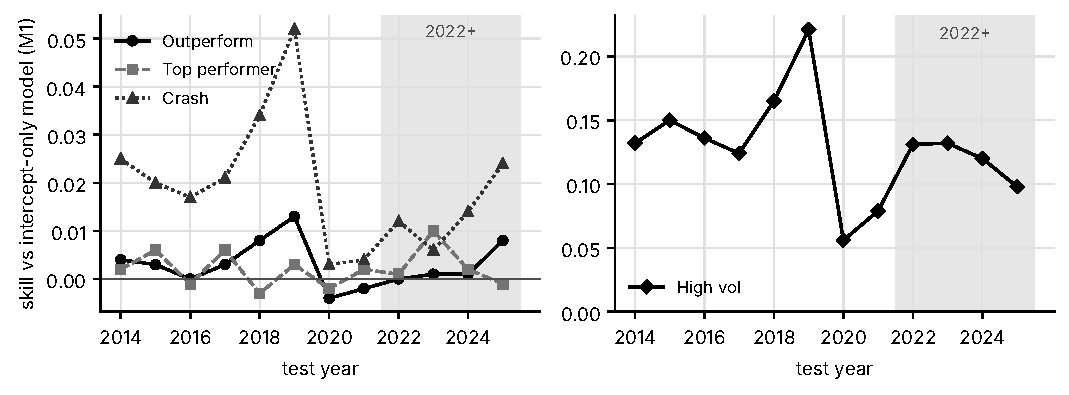
\includegraphics[width=0.9\linewidth]{figures/fig1_skill_by_year.pdf}
\caption{Out-of-sample M1 skill by test year. Left: the three return events. Right: high volatility (different scale). The shaded years 2022--2025 lie in the period the wider project had reserved as a hold-out. Values are parsed from the Phase~2 notebook output (rounded to 3 decimals); no per-year intervals were computed.}
\label{fig:skill}
\end{figure}

\paragraph{How much of the volatility result is persistence? (post hoc).} As a no-fit baseline, I ranked stocks on each test date by their current 60-day realised volatility and computed the per-date AUC for each event on the same test cards. Differences from the classifier use a paired 3-month moving-block bootstrap ($B=1000$). For high volatility, current volatility alone reached an AUC of 0.757, against 0.763 for the M2 classifier. The difference, $+0.006$ (95\% CI $[+0.003, +0.009]$), is real but small. The high-volatility result therefore mostly reflects the persistence of volatility, with the other four features adding a little. The same baseline matched the crash classifier (0.596 against 0.596; difference $-0.0005$, CI $[-0.004, +0.003]$) and the top-performer classifier (0.537 against 0.537; CI $[-0.013, +0.010]$). For these events too, the fitted model's ranking is essentially a volatility ranking. For outperform, current volatility ranks in the wrong direction (AUC 0.471, so ranking low-volatility stocks first gives 0.529, against the model's 0.537); no interval was computed for that reversed comparison. An earlier sandbox analysis of monthly volatility states gives a consistent picture: a stock in the top volatility quintile in one month was in it the next month with probability 0.426, against a 0.20 base rate.

\begin{table}[t]
\centering\small
\caption{M1 odds ratio per one cross-sectional standard deviation: median across the 12 folds, with the number of folds in which the odds ratio exceeded 1 in brackets. Test years 2014--2025.}
\label{tab:odds}
\begin{tabular}{@{}lccccc@{}}
\toprule
Event & Momentum & Reversal & Realised vol & Log-turnover & Overnight drift\\
\midrule
Outperform & 1.094 [12] & 1.002 [6] & 0.892 [0] & 0.994 [5] & 0.975 [0]\\
Top performer & 1.095 [12] & 1.006 [6] & 1.110 [12] & 0.970 [4] & 0.992 [5]\\
Crash & 0.897 [0] & 0.999 [6] & 1.388 [12] & 1.031 [8] & 1.043 [12]\\
High vol & 0.912 [3] & 0.936 [3] & 2.597 [12] & 0.920 [1] & 1.093 [12]\\
\bottomrule
\end{tabular}
\end{table}

Table~\ref{tab:odds} shows the coefficients as a diagnostic. Realised volatility had the largest and most stable coefficients: it raised the odds of high volatility ($2.6\times$ per SD) and of crash ($1.39\times$) in all 12 folds. Momentum raised the odds of outperforming and of a top-quintile return in all 12 folds and lowered crash odds in all 12. Reversal changed sign across folds for every event. Overnight drift raised crash and high-volatility odds in all 12 folds. The top-performer model loaded positively on both momentum and volatility, which is consistent with volatility feeding both tails of the return distribution.

\subsection{From scores to portfolios}

\begin{table}[t]
\centering\small
\caption{Monthly-rebalanced equal-weight portfolios: 141 invested months, January 2014 -- December 2025 (April--June 2025 sat out). All figures are gross of costs. Sharpe is the monthly mean over the monthly SD $\times\sqrt{12}$, with no risk-free rate. Turnover is one-way per month. The last column, turnover $\times2\times12\times0.2\%$, is illustrative and not deducted.}
\label{tab:perf}
\begin{tabular}{@{}lrrrrrr@{}}
\toprule
Portfolio & CAGR & Vol & Sharpe & Max DD & Turnover & Cost line/yr\\
\midrule
Baseline (all stocks) & 12.6\% & 21.3\% & 0.668 & $-45.4\%$ & 0.017 & 0.1\%\\
\addlinespace
Pick outperformers (model) & 17.9\% & 16.3\% & 1.100 & $-26.4\%$ & 0.350 & 1.7\%\\
Pick big winners (model) & 11.4\% & 23.3\% & 0.586 & $-52.4\%$ & 0.334 & --\\
Avoid crashes (model) & 15.2\% & 19.8\% & 0.822 & $-36.1\%$ & 0.085 & 0.4\%\\
Avoid wild movers (model) & 14.9\% & 19.7\% & 0.808 & $-37.5\%$ & 0.080 & 0.4\%\\
\addlinespace
Comparator: cut most volatile & 14.8\% & 20.0\% & 0.797 & $-37.0\%$ & 0.080 & 0.4\%\\
Comparator: momentum $-$ volatility & 21.3\% & 17.2\% & 1.219 & $-25.2\%$ & 0.286 & 1.4\%\\
Reference: momentum only & 19.6\% & 20.7\% & 0.978 & $-29.8\%$ & 0.226 & 1.1\%\\
\bottomrule
\end{tabular}
\end{table}

Both avoid portfolios passed the pre-committed ``reduces risk'' and ``worth it'' rules (Table~\ref{tab:perf}, Figure~\ref{fig:sharpe}). Their volatility-difference CIs were $[-1.94, -1.15]$ and $[-1.96, -1.21]$ percentage points, and their Sharpe-difference CIs $[+0.085, +0.258]$ and $[+0.075, +0.237]$. Both Sharpe gains held at 98.75\%. Neither pick portfolio passed ``adds return''. Pick outperformers earned $+3.72\%$/yr of active return, with CI $[-1.60\%, +8.67\%]$ and halves of $+6.0\%$ and $+1.3\%$. Its Sharpe advantage ($[+0.209, +0.726]$) came mainly from lower volatility (16.3\% against 21.3\%). These Sharpe gains come from long-only, absolute-return portfolios. A portfolio holding calmer stocks can raise its Sharpe ratio through lower market exposure without better relative selection. Because betas and factor exposures were not estimated, the gains should not be read as stock-selection alpha. Both avoid portfolios' active returns fell from about 3\%/yr in 2014--19 to under 0.6\%/yr in 2020--25.

\begin{figure}[t]
\centering
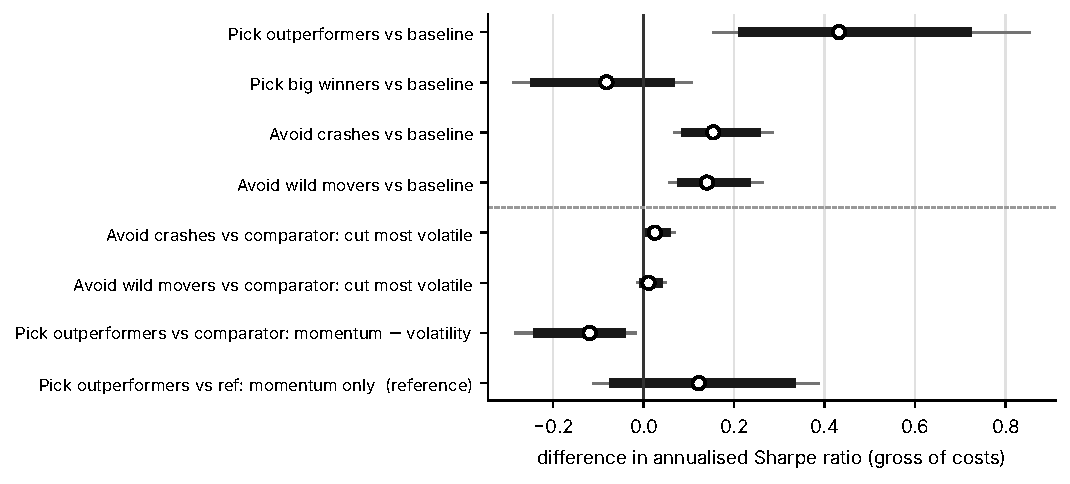
\includegraphics[width=0.88\linewidth]{figures/fig2_sharpe_diff.pdf}
\caption{Differences in annualised Sharpe ratio, gross of costs, over 141 months (2014--2025, including the 2022--2025 hold-out period). Intervals come from a paired moving-block bootstrap (6-month blocks, $B=2000$). Thick bars are 95\% intervals. Thin bars are 98.75\% above the dashed line (four comparisons with the baseline) and 98.33\% below it (three pairs). Above the line: model portfolio minus baseline, with points equal to differences of the reported Sharpe ratios. Below the line: model minus the hindsight-designed comparator.}
\label{fig:sharpe}
\end{figure}

\subsection{Model versus comparator}

\begin{table}[t]
\centering\small
\caption{Characteristics of the model portfolios: mean within-date z-score of held stocks over 141 months, and the mean (minimum) monthly share of the model's holdings that the comparator also held. Two random 80\% subsets overlap about 80\%; two random 20\% subsets overlap about 20\%.}
\label{tab:tilt}
\begin{tabular}{@{}lrrrrrl@{}}
\toprule
Portfolio & Mom & Rev & Vol & Turn & Overn. & Overlap with comparator\\
\midrule
Pick outperformers & $+0.83$ & $-0.01$ & $-0.64$ & $+0.19$ & $-0.39$ & 74.3\% (48.0\%) mom$-$vol\\
Pick big winners & $+0.96$ & $+0.07$ & $+1.07$ & $+0.11$ & $+0.13$ & --\\
Avoid crashes & $+0.06$ & $-0.04$ & $-0.36$ & $-0.02$ & $-0.11$ & 95.8\% (92.3\%) cut-vol\\
Avoid wild movers & $0.00$ & $-0.02$ & $-0.37$ & $+0.01$ & $-0.10$ & 96.9\% (93.2\%) cut-vol\\
\bottomrule
\end{tabular}
\end{table}

Table~\ref{tab:tilt} shows why simple comparators were the natural benchmark. The stocks held by the avoid portfolios had mean volatility z-scores of $-0.36$ and $-0.37$, so the excluded fifth averaged about $+1.45$. Of the stocks excluded by avoid crashes, 86.2\% (minimum 73.7\%) were also excluded by avoid wild movers. The two prediction rankings had an average rank correlation of 0.93. Pick outperformers sat in the high-momentum, low-volatility corner.

The three pre-committed pairs (lower panel of Figure~\ref{fig:sharpe}):
\begin{itemize}
\item \textbf{Avoid crashes vs.\ cut most volatile:} $+0.025$, 95\% CI $[+0.003, +0.060]$, 98.33\% CI $[-0.001, +0.068]$. The model passes the unadjusted 95\% rule, so the result is marginal at 95\%, and it is not robust to the three-comparison interval. Active return was $+0.33\%$/yr with CI $[-0.13\%, +0.91\%]$.
\item \textbf{Avoid wild movers vs.\ cut most volatile:} $+0.011$, 95\% CI $[-0.008, +0.041]$, so there is no detectable difference.
\item \textbf{Pick outperformers vs.\ momentum $-$ volatility:} $-0.119$, 95\% CI $[-0.244, -0.040]$, 98.33\% CI $[-0.283, -0.019]$, so under the pre-committed rule the comparator is better. Active return was $-3.01\%$/yr with CI $[-4.92\%, -1.60\%]$, negative in both halves. Because the comparator was designed after the model's tilts were observed, this shows only that, over this sample, a 1:1 combination of the two characteristics the model leaned on did at least as well as the fitted weights. It does not show that the comparator would beat the model going forward.
\end{itemize}
In the reference comparison with momentum only, the model's Sharpe was higher by $+0.122$ (95\% CI $[-0.076, +0.336]$), which is inconclusive. All three comparators beat the baseline on Sharpe: cut most volatile $[+0.071, +0.210]$, momentum $-$ volatility $[+0.306, +0.893]$ and momentum only $[+0.073, +0.592]$. Before the run, the notebooks expected the avoid pairs to show high overlap and little difference, which they did, and expected pick outperformers to tie its comparator, which it did not.

%------------------------------------------------------------------------------
\section{Robustness and diagnostics}
\label{sec:robust}

\paragraph{Leakage and reproduction.} Each prediction lies in its own fold's test year. A fresh fit of the 2019 crash model on pre-2019 rows reproduced the stored predictions exactly. Three forward returns recomputed from raw opens matched the dataset exactly. Portfolio and comparator returns for two months matched an independent recomputation to $10^{-12}$, and each phase reproduced the previous one. On the M0 rung, intercepts equalled the logit of the training base rate and AUC was 0.500.

\paragraph{Universe and survivorship.} None of the 68,670 candidate stock-months had a flag other than 1. For example, 63MOONS.NS was excluded after leaving the index on 2017-01-02. Twenty-three stock-months (0.033\%) lacked a forward return (median return to the last price $+3.0\%$). Adjacent holding windows overlapped by 0.29 days on average (maximum 3), so monthly returns are close to non-overlapping.

\paragraph{Absolute versus relative target (verified diagnostics).}\label{sec:absolute}
Two earlier sandbox notebooks fitted ordinary least squares on the same features and folds, one to the absolute target and one to the target minus that date's equal-weighted mean (outputs re-extracted for this revision). For the absolute target, the mean across the 12 folds of the per-fold out-of-sample $R^2$ was $-0.0421$. The mean across folds of the per-date Spearman rank IC was $+0.0540$, and the IC was positive on 65\% of dates. When the date mean was subtracted from the target, mean $R^2$ became $+0.0003$, while the rank IC was unchanged to four decimals in every fold, as it must be: subtracting a per-date constant cannot reorder stocks. The date-mean component accounted for 28.6\% of the pooled variance of the target over all cards from 2011 to 2026. These descriptive diagnostics, which carry no intervals, motivate the within-date rank labels.

%------------------------------------------------------------------------------
\section{Limitations}
\label{sec:limits}
\begin{enumerate}
\item \textbf{No project-level hold-out.} Every number uses 2014--2025 test years, and training windows and design choices drew on 2022--2025 (Section~\ref{sec:holdout}).
\item \textbf{Hindsight comparator.} The momentum-minus-volatility rule was chosen after the Phase~3a tilts were seen. Its 21.3\% CAGR and 1.22 Sharpe are not evidence of a prospective strategy. Momentum \citep{jegadeesh1993} and low volatility \citep{ang2006} are long-established characteristics, which makes the rule plausible but does not remove the hindsight.
\item \textbf{Post hoc inference.} The moving-block intervals, the volatility baseline and the feature-geometry distributions were added in revision, after the original results were known. The outperform rule-1 verdict depends on block length; I treat the 3-month specification, chosen before the rerun, as primary.
\item \textbf{Costs, capacity and exposures.} All returns are gross. The illustrative cost line is about 1.7\%/yr for pick outperformers, about half its gross active return. Spreads, market impact and capacity of equal-weighted small caps were not modelled. Market beta and factor exposures were not estimated, so lower market exposure may contribute to every Sharpe gain reported.
\item \textbf{Multiple comparisons and selection.} The 15 \texttt{SBX} verdicts, and several unrecorded looks at the same 2014--2025 sample in earlier sandbox stages, mean that only results surviving the wider intervals should be treated as established. A deflated-Sharpe adjustment \citep{bailey2014} was not computed.
\item \textbf{Specification.} The models are unregularised; regularisation is outside this paper's scope. The training objective (log-loss for an event across all stocks) differs from the portfolio's use of the scores (top-quintile ranking). This is one plausible, untested reason the fitted weights trailed the 1:1 rule. Others are estimation noise from annual three-year refits and weight placed on noisy features.
\item \textbf{Data.} April--June 2025 is missing, and the exchange-closed-date issue is unresolved (Section~\ref{sec:data}). The July--December 2018 universe may be misclassified.
\end{enumerate}

\paragraph{What this paper does not establish.} It does not show that any of these portfolios would be profitable after costs, that the momentum-minus-volatility rule would beat a fitted model on future data, or that the Sharpe gains are stock-selection alpha rather than lower market exposure. It does not show that the five features are uncorrelated on every date (they are not), or that fitted classifiers are generally inferior to simple rules beyond these five features, labels, universe and folds. Failure to detect a difference, as for avoid wild movers, is not evidence that no difference exists.

%------------------------------------------------------------------------------
\section{Conclusion}
Across the tested rolling folds, the five-characteristic logistic models contained little information about which stocks would beat the cross-sectional median; under the post hoc moving-block intervals, the outperform skill is not distinguishable from zero. Relative future volatility was substantially more predictable, mostly because volatility persists: ranking by current volatility alone came within 0.006 AUC of the fitted model. The avoid portfolios largely reproduced a simple exclusion of the most volatile fifth. Their incremental Sharpe advantage over that rule was small, marginal at 95\% for the crash model, and not robust to the three-comparison interval. The outperform portfolio did not beat the momentum-minus-volatility comparator, which was designed with hindsight. The sample includes the project's previously reserved hold-out, the volatility feature has a documented missing-data episode, the portfolio results are gross of costs, and exposures were not estimated. The findings are therefore diagnostic, not prospective evidence of a tradable strategy. The next steps are exposure regressions for the portfolios and a frozen-protocol forward test of the fitted model and the comparator.

\section*{Reproducibility}
\begin{table}[h]
\centering\footnotesize
\setlength{\tabcolsep}{3pt}
\begin{tabularx}{\linewidth}{@{}lX@{}}
\toprule
Item & Setting\\
\midrule
Dataset & \texttt{ml\_sandbox\_v1\_dataset\_2026-09-07}: 1,813,407 cards, 3,756 dates, 2011-01-03 to 2026-06-10\\
Phase 2 (2026-09-30) & 12 folds, 3 y / 1 y, 21-date purge; 1,411,188 test cards (high vol 1,411,156); scikit-learn \texttt{LogisticRegression}, no penalty, L-BFGS; original i.i.d.\ month bootstrap $B=1000$, seed 0\\
Phase 3a/3b (2026-10-04/05) & 141 rebalances (Apr--Jun 2025 sat out), median 490 stocks; paired 6-month moving blocks, $B=2000$, seed 0; 95\%, 98.75\% (3a), 98.33\% (3b)\\
Revision (post hoc) & run 2026-10-14; gate reproduced all 36 published i.i.d.\ values; blocks 2/3/6 of 142 months, $B=1000$, seeds 20261016/17/20; volatility baseline paired 3-month blocks, seed 314; geometry on 3,756 dates\\
Software & Python 3 on Colab; library versions not recorded\\
\bottomrule
\end{tabularx}
\end{table}

\aistatement
{\sloppy\availability{\ghbase/indian-equity-research/tree/main/p4_models_vs_rules}\par}

\renewcommand{\bibfont}{\small}
\bibliographystyle{plainnat}
\bibliography{../common/refs}

\end{document}
